\section {Implementation with POSIX shared memory and RDMA}


  \begin{figure*}
    \centering
    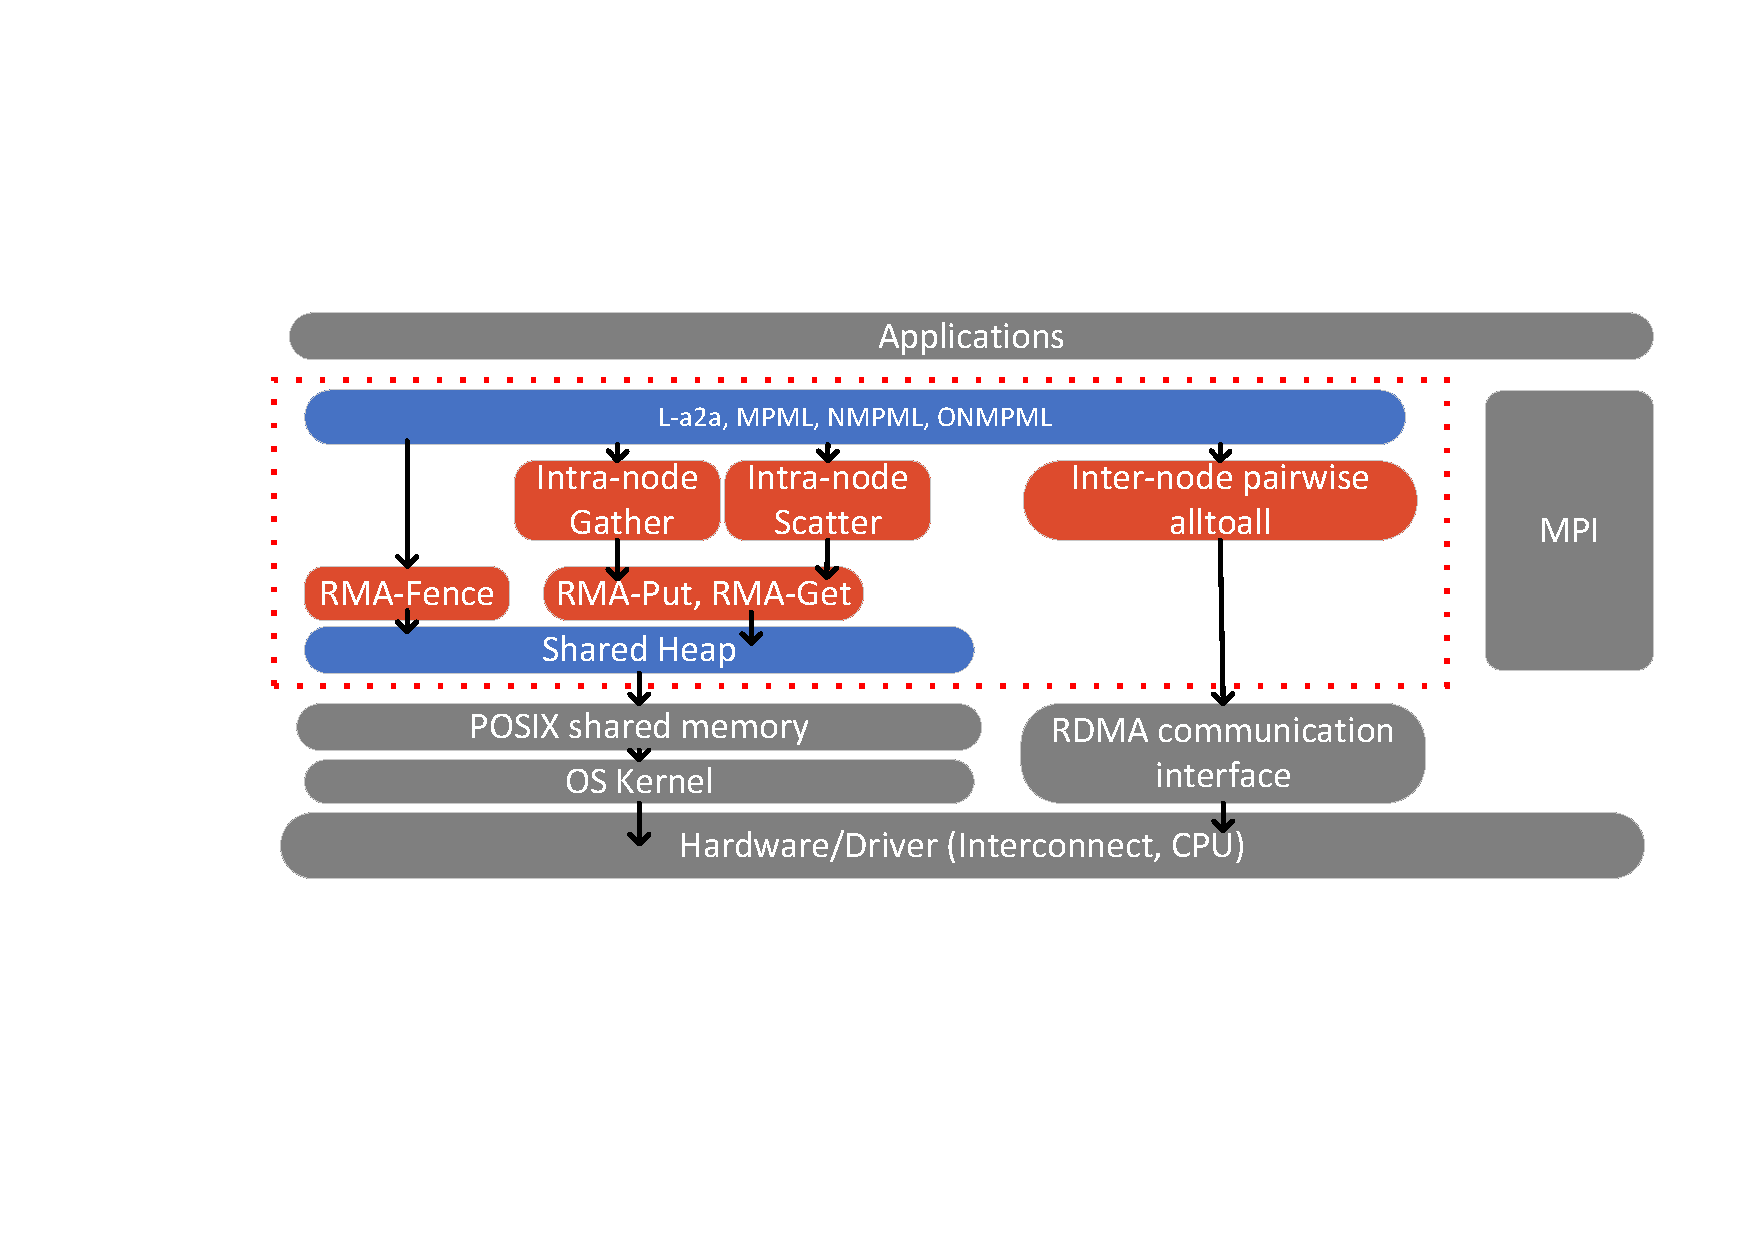
\includegraphics[width=16cm]{./Figures/implementaion.pdf} %[图片大小]{图片路径}
    \caption{Implementation overview.} %图片标题
    \label{fig:Implementation}
    \end{figure*}


As shown in Figure ~\ref{fig:Implementation}, the dash box include our impementation parts.
Our implemtation is based on shared memory and Galaxy Express (GLEX) communication layer (to support RDMA) for Tianhe series network.

\subsection {Impementation of Intra-node Communication}
Shared Heap \cite{friedley2013hybrid} is a large free shared memory  created by POSIX interface.
Then, each processes in a node associative the shared memory into its own addres space.
After that, a reimplented malloc (glex-malloc) which allocated the memory on this shared memory.
The memory allocated by glex-malloc are accessable by all ranks in a same node.
User's application must using glex-malloc to allocate sendbuf and recvbuf of all-to-all communication.
As a result, each processes in the node, can directly access the memory allocate on shared heap.

There is a set of intra-node operations RMA-fence, RMA-Put,and RMA-Get which based on shared heap. 
They are similar to MPI-Win-fence, MPI-Put and MPI-Get.
RMA-fence is a intra-node fence.
Between two RMA-fence, all ranks in a node is free to access other ranks buffer with RMD-Put and RMA-Get.
Difference is that a rank call RMA-Put or RMA-Get is blocking communication.
When  RMA-Put or RMA-Get return, the data is actually moved from one rank to another rank.


\subsection {Impementation of Inter-node Communication}

In gather-scatter-based all-to-all, the messages are aggregated. 
For most cases, they are large message.
In MPI, there are  eager protocol for small message and rendezvous protocol for large message.
Rendenzvous protocal have a "rendenzvous start" and "rendenzvous fin" overhead for each large message sending.
To avoid these protocal overhead, we directly use Remote Direct Memory Access (RDMA) to do inter-node communication.
RDMA communication must based on preregisted buffer.
This paper using two pre-registered buffer (BufferSend, BufferRecv) on each node to do inter-node RDMA.
Gathering operation direct gather the data on to BufferSend, than start RDMA communication. 
After receiver rank detect a receive event, it transpose the data and directly scatter the data on to receive buffer.
RDMA-based communication do not need  "rendenzvous start" and "rendenzvous fin" overhead for each large message transmission.
This avoids the overhead caused by the rendenzvous protocol.